%%%%%%%%%%%%%%%%%%%%%%%%%%%%%%%%%%%%%%%%%
% Thin Sectioned Essay
% LaTeX Template
% Version 1.0 (3/8/13)
%
% This template has been downloaded from:
% http://www.LaTeXTemplates.com
%
% Original Author:
% Nicolas Diaz (nsdiaz@uc.cl) with extensive modifications by:
% Vel (vel@latextemplates.com)
%
% License:
% CC BY-NC-SA 3.0 (http://creativecommons.org/licenses/by-nc-sa/3.0/)
%
%%%%%%%%%%%%%%%%%%%%%%%%%%%%%%%%%%%%%%%%%

%----------------------------------------------------------------------------------------
%	PACKAGES AND OTHER DOCUMENT CONFIGURATIONS
%----------------------------------------------------------------------------------------

\documentclass[a4paper, 12pt]{article} % Font size (can be 10pt, 11pt or 12pt) and paper size (remove a4paper for US letter paper)
\usepackage[top=1in, bottom=1.25in, left=1in, right=1in]{geometry}
\usepackage[protrusion=true,expansion=true]{microtype} % Better typography
\usepackage{graphicx} % Required for including pictures
\usepackage{wrapfig} % Allows in-line images
\usepackage{caption}
\usepackage{amsmath}
\usepackage{mathtools}
\usepackage{float}
\usepackage{mathpazo} % Use the Palatino font
\usepackage[T1]{fontenc} % Required for accented characters
\linespread{1.05} % Change line spacing here, Palatino benefits from a slight increase by default

\makeatletter
\renewcommand\@biblabel[1]{\textbf{#1.}} % Change the square brackets for each bibliography item from '[1]' to '1.'
\renewcommand{\@listI}{\itemsep=0pt} % Reduce the space between items in the itemize and enumerate environments and the bibliography

\renewcommand{\maketitle}{ % Customize the title - do not edit title and author name here, see the TITLE block below
\begin{flushright} % Right align
{\LARGE\@title} % Increase the font size of the title

\vspace{50pt} % Some vertical space between the title and author name

{\large\@author} % Author name
\\\@date % Date

\vspace{40pt} % Some vertical space between the author block and abstract
\end{flushright}
}

%----------------------------------------------------------------------------------------
%	TITLE
%----------------------------------------------------------------------------------------

\title{\textbf{\'Atomo de Hidrogeno relativista}\\ % Title
La perspectiva de Dirac} % Subtitle

\author{\textsc{Juan David Orjuela Zu\~niga \\ Juan Nicol\'as Garavito Camargo} % Author
\\{\textit{Departamento de F\'isica\\}
\textit{Universidad de los Andes, Bogot\'a, Colombia}}} % Institution

\date{\today} % Date

%----------------------------------------------------------------------------------------

\begin{document}

\maketitle % Print the title section

%----------------------------------------------------------------------------------------
%	ABSTRACT AND KEYWORDS
%----------------------------------------------------------------------------------------

%\renewcommand{\abstractname}{Summary} % Uncomment to change the name of the abstract to something else

\begin{abstract}
Resumen, JD \& JN
\end{abstract}
\hspace*{3,6mm}\textit{Keywords:}  % Keywords

\vspace{30pt} % Some vertical space between the abstract and first section

%----------------------------------------------------------------------------------------
%	ESSAY BODY
%----------------------------------------------------------------------------------------

\section{Antecedentes historicos}


La mec\'anica cu\'antica tiene una particularidad entre los diferentes cuerpos te\'oricos de las ramas de la f\'isica. A diferencia de la mec\'anica newtoniana o la relatividad especial, desarrolladas por Newton y Einstein respectivamente, la mec\'anica cu\'antica tiene muchos padres y una historia accidentada y llena de baches. Ni siquiera la electrodin\'amica tiene esa caracter\'istica, pues, a pesar de ser el producto del trabajo conjunto de muchos hombres de ciencia, fue "empaquetada" y sintetizada en su forma actual por Maxwell. Esto les da una cierta unidad: un orden y caracter l\'ogico propio de ser el producto de una sola mente. El ep\'itome de esa naturaleza est\'a condensado en la famosa frase de Richard Feynman en que seguraba estar convencido de que nadie realmente entiende la mec\'anica cu\'antica. Pero eso no ha impedido el avance de esta rama de la f\'isica. Si bien no hay un consenso general sobre sus postulados o lo que significa, la mec\'anica cu\'antica ha avanzado de forma inimaginable desde sus ca\'oticos or\'igenes, siendo la ecuaci\'on de Schr\"odinger uno de sus pilares (un postulado, en otras famosas palabras de Feynman: "Where did we get that (equation) from? Nowhere. It is not possible to derive it from anything you know. It came out of the mind of Schr\"odinger").

La cuantizaci\'on de la luz de Planck junto con a la interpretaci\'on de Einstein llev\'o a de Broglie a proponer su relaci\'on entre el n\'umero de onda y el momento, inspir\'andose en la relatividad especial. Debye entonces propuso que si las part\'iculas se comportaban como ondas entonces deber\'ian obedecer alg\'un tipo de ecuaci\'on de onda, lo que inspir\'o a Schr\"odinger a buscar una ecuaci\'on de onda tridimensional apropiada para el electr\'on, lo que lo llev\'o a encontrar la ecuaci\'on

\begin{equation}
i\hbar\frac{\partial}{\partial t} \psi (\vec{r}, t)=-\frac{\hbar^2}{2m}\nabla^2  \psi (\vec{r}, t) + V(\vec{r}) \psi (\vec{r}, t)
\end{equation}

Luego de esto Sch\"odinger us\'o la relaci\'on relativista entre momento y energ\'ia para derivar lo que conocemos ahora como la ecuaci\'on de Klein-Gordon para potencial coulombiano. Pero dado que sus correcciones relativistas no cuadraban bien con los resultados de Sommerfeld decidi\'o abandonar esa idea y dejar las correciones relativistas para despu\'es, dedic\'andose a encontrar exitosamente los niveles de energ\'ia del modelo de Bohr sin estructura fina para la serie espectral del hidr\'ogeno. 

Curiosamente, la ecuaci\'on de Klein-Gordon fue descubierta antes de la de  Sch\"odinger y aunque la ecuaci\'on de Klein-Gordon se interpreta como una versi\'on relativista de la ecuaci\'on de Sch\"odinger, no se puede hacer el an\'alogo directamente por dos motivos principales: tiene segunda derivada temporal y no conserva densidad de probabilidad. Sus autores propusieron que describ\'ia electrones relativistas, pero dado que no tiene en cuenta el spin del electr\'on hace predicciones incorrectas para la estructura fina del \'atomo de hidr\'ogeno, sobreestimando el patr\'on de desdoblamiento de las l\'ineas.

Ser\'ia Dirac quien, seg\'un cuenta una leyenda, mientras observaba una fogata en una noche de 1928 se dio cuenta que necesitaba una ecuaci\'on de onda relativista linear en el espaciotiempo. Para esto tambi\'en necesit\'o partir de la relaci\'on relativista entre energ\'ia y momento. Lo que obtuvo qued\'o plasmado en los anales de la historia de la ciencia por sus poderosas implicaciones. Siendo la primera teor\'ia en tener en cuenta completamente la relatividad especial en el contexto mec\'anico cu\'antico, pudo hacer un tratamiento riguroso del espectro del \'atomo de hidr\'ogeno. Adem\'as de eso, predijo la existencia de la antimateria, algo de lo que no se ten\'ia ning\'un tipo de evidencia experimental hasta ese momento. Y por si eso fuera poco, provee una justificaci\'on te\'orica a las propuestas fenomenol\'ogicas que hizo Pauli para el spin, mostrando que es una consecuencia del matrimonio entre relatividad y mec\'anica cu\'antica. Las consecuencias se sienten hasta el d\'ia de hoy, en que, en el contexto de teor\'ia cu\'antica de campos, la soluci\'on a la ecuaci\'on ya no interpretar\'ia como una "onda" sino como un "campo", un campo cu\'antico correspondiente a las part\'iculas de spin 1/2.


% ------------------------------------- Ecuacion de Dirac --------------------------------------
\section{Ecuaci\'on de Dirac}
La ecuaci\'on de Dirac al igual que la ecuaci\'on de Klein-Gordon es una 
ecuaci\'on relativista de la mec\'anica cuantica. Adem\'as tiene en cuenta
part\'iculas de sp\'in $s=1/2$ tales como electrones, protones, neutrones etc. 

En esta secci\'on se derivara la ecuaci\'on de Dirac mediante argumentos
de simetr\'ia (mostrando as\'i una manera alternativa a la vista en clase). 
Una ecuaci\'on relativista debe ser simetrica tanto en el tiempo como en el 
espacio, esto debido a que el tiempo y el espacio son una misma cantidad 
en las transformaciones de Lorentz.

Es conocido de relatividad especial que la energ\'ia de una part\'icual esta dada
por:

\begin{equation}
E^2 = m^2c^4 + p^2c^2
\end{equation}

Si expresamos $E$ y $p$ como operadores obtenemos la ecuaci\'on de Klein-Gordon:

\begin{equation}
\left( \nabla^2 - \dfrac{1}{c^2}\dfrac{\partial^2}{\partial t^2} - \dfrac{m^2c^2}{\hbar^2}   \right)\psi(\mathbf{r}, t) = 0
\end{equation} 


Sin embargo una forma a\'un mas general ser\'ia permitir a la funci\'on de onda tener $N$ componentes. La forma mas 
general posible para la derivida temporal de la ecuaci\'on de onda \cite{dirac1,dirac2}:

\begin{equation}\label{eq:dirac1}
\dfrac{1}{c}\dfrac{\partial \psi_i(\mathbf{r},t)}{\partial t} =
- \sum \limits_{k=x,y,z} \sum \limits_{n=1}^{N}\alpha^k_{i,n} \dfrac{\partial \psi_n}{\partial k} -
\dfrac{imc}{\hbar}\sum \limits_{n=1}^{N}\beta_{i,n}\psi_n(\mathbf{r}, t)
\end{equation}

Donde el primer termino del lado derecho corresponde a la contribucion 
de todas las derivadas espaciales de todas las componentes de la funci\'on 
de onda y el segundo termino es una combinacion lineal de todas las 
componentes de $\psi$. $\alpha$ y $\beta$ son constantes que hacen que la 
ecuaci\'on tenga las dimensiones correctas. (\ref{eq:dirac1}) puede escribirse
de forma matricial haciendo la suma de todas las componentes $N$.   

\begin{equation}\label{dirac}
i\hbar \partial_t \psi(\mathbf{r},t) = \hat{\mathbf{H}}\psi(\mathbf{r},t) =
(c\widetilde{\alpha}\cdot \hat{\mathbf{p}} + \widetilde{\beta}mc^2)\psi(\mathbf{r},t)
\end{equation}

Donde $\partial_t = \partial / \partial t$ y $\widetilde{\alpha}$ y $\widetilde{\beta}$ son matrices de dimension $N$, 
estas se llaman \textbf{matrices de Dirac}.
Como se vio en clase estas matrices deben satisfacer las siguientes condiciones:\\

\[
\alpha_i^2 = \beta^2 = I \\
\]
\[
\alpha \beta + \beta \alpha = 0 \\
\]
\[
\alpha_j \alpha_i + \alpha_i \alpha_j = 0
\]
\[
i,j=x, y, z\\
\] 

Las matrices que cumplen con estas condiciones para $N=4$ estan definidas en terminos
de las matrices de Pauli:

\begin{equation}
\widetilde{\alpha_i}=
\begin{pmatrix}
0 & \widetilde{\sigma}_i\\
\widetilde{\sigma}_i & 0 \\
\end{pmatrix}
\end{equation}

\begin{equation}
\widetilde{\beta}=
\begin{pmatrix}
\widetilde{\mathbf{I}}_2 & 0\\
0 & -\widetilde{\mathbf{I}}_2 \\
\end{pmatrix}
\end{equation}

Donde $\widetilde{\mathbf{I}}_2$ son matrices unitarias de dimension 2. 
Adicionalmente las matrices de \textbf{spin} de Pauli de 4 dimensiones
estan definidas como:

\begin{equation}
\widetilde{\sigma}_{4i}=
\begin{pmatrix}
\widetilde{\sigma}_i & 0 \\
0 & \widetilde{\sigma}_i  \\
\end{pmatrix}
\end{equation}

Las propiedades de estas matrices se pueden ver en \S$\ref{sec:gamma5}$.

%----------------------- Solucion de el atomo de hidrogeno con Dirac -------------------------

\section{Soluci\'on de la ecuaci\'on de Dirac para el \'atomo de Hidrogeno}

%----------Coordenadas radiales-----------------------

Para el \'atomo de Hidrogeno debemos solucionar (\ref{dirac})
con un potencial $V(r)$ definido como:

\begin{equation}
V(r) = \dfrac{Ze^2}{4\pi\epsilon_0 r^2}
\end{equation}

Con el fin de simplificar la notaci\'on llamaremos una variable
$\xi$ definida como:

\begin{equation}
\xi = \dfrac{Ze^2}{4\pi \epsilon_0 \hbar c}
\end{equation}

La ecuaci\'ond de Dir\'ac para este potencial se expresa como:

\begin{equation}\label{eq:diracvr}
(c \widetilde{\alpha} \cdot \hat{p} + \widetilde{\beta} m c^2 + V(r) ) \phi(r) = E \phi (r)
\end{equation}

Para solucionar esta ecuaci\'on debemos primero transformarla a coordenadas
esfericas. En la siguiente secci\'on se desarrolla en detalle esta transformaci\'on.
El desarrollo matematico realizado en este trabajo sigue el procedimiento 
explicado en \cite{strange}, todos los pasos intermedios son desarrollados con 
detalle en \S \ref{sec:apendice}. 
%---------------------------------Coordenadas esfericas ------------
\subsection{Ecuaci\'on de Dirac en coordenadas esfericas}

En (\ref{eq:diracvr}) el termino que se debe transformar a coordenadas radiales
 es $\widetilde{\alpha} \cdot \hat{\mathbf{p}}$, ya que $\widetilde{\beta}$ es independiente del sistema de coordenadas. 

\begin{equation}\label{eq:alphap}
\widetilde{\alpha} \cdot \hat{\mathbf{p}} = -i \hbar \widetilde{\alpha} \cdot \nabla
\end{equation}

Haciendo uso de la identidad vectorial: 

\begin{equation}\label{eq:identity}
\nabla = \hat{\mathbf{r}}(\hat{\mathbf{r}}\cdot \nabla) - \hat{\mathbf{r}} \times (\hat{\mathbf{r}} \times \nabla)  
\end{equation}

Adem\'as teniendo en cuenta la simetr\'ia esferica del sistema, es decir donde $\partial/\partial \theta = 0$
y $\partial/\partial \phi = 0$,  (\ref{eq:identity}) se puede expresar como:

\begin{equation}\label{eq:nabla1}
\mathbf\nabla = \hat{\mathbf{r}}(\dfrac{\partial}{\partial r}) - \hat{\mathbf{r}} \times (\hat{\mathbf{r}} \times \nabla)
\end{equation}

El segundo termino en (\ref{eq:nabla1}) se puede expresar en terminos del momento angular $\mathbf{L} = -i\hbar \mathbf{r} \times \mathbf{\nabla}$.
as\'i:

\begin{equation}\label{eq:nabla}
\mathbf{\nabla} =  \hat{\mathbf{r}}(\dfrac{\partial}{\partial r}) - \dfrac{i}{\hbar}\dfrac{\hat{\mathbf{r}}}{r} \times \mathbf{L}
\end{equation}

Por lo tanto (\ref{eq:alphap}) se puede escribir en terminos de (\ref{eq:nabla}) como:

\begin{equation}\label{eq:alphap2}
\widetilde{\alpha}\cdot \mathbf{\hat{p}} = -i\hbar \widetilde({\alpha}\cdot \hat{\mathbf{r}}(\dfrac{\partial}{\partial r}) - 
\dfrac{i}{\hbar}\widetilde{\alpha}\cdot \dfrac{\hat{\mathbf{r}}}{r} \times \mathbf{L})
\end{equation}

El \'ultimo termino de la derecha de (\ref{eq:alphap2}) se puede expresar como:

\begin{equation}\label{eq:prop1}
\widetilde{\alpha}\cdot\hat{\mathbf{r}}\widetilde{\alpha} \cdot \hat{\mathbf{L}} = i\widetilde{\sigma}\cdot \hat{\mathbf{r}} \times \mathbf{L}
\end{equation}

En donde se uso la relaci\'on:

\begin{equation}
\widetilde{\alpha}\cdot \hat{\mathbf{A}}\widetilde{\alpha}\cdot \hat{\mathbf{B}}
= \hat{\mathbf{A}} \cdot \hat{\mathbf{B}} +  i\widetilde{\sigma}\cdot \hat{\mathbf{A}}\times \hat{\mathbf{B}}
\end{equation}

Donde $\hat{\mathbf{A}}$ y $\hat{\mathbf{B}}$ son vectores arbitrarios, 
multiplicando a ambos lados de (\ref{eq:prop1}) por $\gamma_5$ (ver \S \ref{sec:gamma5}) 
obtenemos:   

\begin{equation}
i\widetilde{\alpha}\cdot\hat{\mathbf{r}}\widetilde{\sigma} \cdot \hat{\mathbf{L}} = -\widetilde{\alpha}\cdot \hat{\mathbf{r}} \times \mathbf{L}
\end{equation}

Por lo tanto (ref{eq:alphap2}) se puede escribir como:

\begin{equation}\label{eq:alphap3}
\widetilde{\alpha}\cdot \mathbf{\hat{p}} = -i\hbar \widetilde{\alpha}\cdot \hat{\mathbf{r}}\partial_r + \dfrac{i}{|\mathbf{r}|}
\widetilde{\alpha}\cdot \hat{\mathbf{r}}\widetilde{\sigma}\cdot \hat{\mathbf{L}}
\end{equation} 

Finalmente escribiendo el ultimo termino de (\ref{eq:alphap3}) en terminos
del vector $\hat{K}$ (Ver pasos intermedios en \S \ref{sec:k}) se obtiene:

\begin{equation}\label{alphap4}
\widetilde{\alpha} \cdot \mathbf{\hat{p}} = -i\hbar \widetilde{\alpha}\cdot \hat{\mathbf{r}}\partial_r + \dfrac{i}{|\mathbf{r}|} \widetilde{\alpha_r}(\widetilde{\beta}\hat{K}-\hbar)
\end{equation}

Reemplazando este resultado en (\ref{eq:diracvr}) se obtiene la ecuaci\'on de Dirac en coordenadas esfericas.

\begin{equation}\label{eq:radialdirac}
\left (ic\widetilde{\gamma_5}\widetilde{\sigma_r} \left (\hbar \partial_r + \dfrac{\hbar}{r} -  \dfrac{\widetilde{\beta}\hat{K}}{r}\right )  + \widetilde{\beta} m c^2 + V(r) \right ) \phi(r) = E \phi (r)
\end{equation}

Vamos entonces a insistir que nuestro autoestado de 4 componentes sea lo m\'as parecido posible a los espinores de dos componentes de Pauli:

\begin{equation}\label{eq:funciondeonda}
\phi^{m_j}_{\kappa} (\vec{r} ) = \left( \substack{g_{\kappa}(r)\chi^{m_j}_\kappa (\hat{r}) \\ if_\kappa(r)\chi^{m_j}_{-\kappa} (\hat{r}) } \right) 
\end{equation}

En donde $\chi_{\kappa}^{mj}$ son funciones spin-angulares. Es importante
recordar que en el caso relativista las funciones radiales cambian y 
cuando tenemos en cuenta el sp\'in se introducen los spinores de Pauli
en la funci\'on de onda. Substituyendo (\ref{eq:funciondeonda}) en 
(\ref{eq:radialdirac}) se encuentran 4 ecuaciones de las cuales 2 son 
separables:
 

\begin{equation}
-c \hbar  \left( \frac{\partial}{\partial r}+\frac{1}{r}+\frac{\kappa}{r} \right) g_{\kappa}(r)\chi^{m_j}_{-\kappa} +(E-V(r)+mc^2)f_{\kappa}(r)\chi^{m_j}_{-\kappa}
\end{equation}


\begin{equation}
c \hbar  \left( \frac{\partial}{\partial r}+\frac{1}{r}+\frac{\kappa}{r} \right) f_{\kappa}(r)\chi^{m_j}_{\kappa} +(E-V(r)-mc^2)g_{\kappa}(r)\chi^{m_j}_{\kappa}
\end{equation}


Lo que permite cancelar el t\'ermino $\chi^{m_j}_{\kappa}$ y ver que el 
imaginario puro de las soluciones tiene el papel de asegurar que la parte 
radial de la autofunci\'on es real. Se pueden reescribir entonces como:


\begin{equation}
\frac{\partial g_{\kappa}(r)}{\partial r} =\frac{\kappa+1}{r}g_{\kappa}(r)+\frac{1}{c\hbar}(E-V(r)+mc^2)f_{\kappa}(r)
\end{equation}

\begin{equation}
\frac{\partial f_{\kappa}(r)}{\partial r} =\frac{\kappa-1}{r}f_{\kappa}(r)-\frac{1}{c\hbar}(E-V(r)-mc^2)g_{\kappa}(r)
\end{equation}

Que es la forma usual de la ecuaci\'on de radial de Dirac. Sin embargo, a menudo es \'util hacer los reemplazos $u_{\kappa}(r)=rg_{\kappa}(r)$ y $v_{\kappa}(r)=rg_{\kappa}(r)$, lo que permite que la ecuaci\'on se vea as\'i


\begin{equation}\label{eq:rad1}
\frac{\partial u_{\kappa}(r)}{\partial r} =-\frac{\kappa}{r}u_{\kappa}(r)+\frac{1}{c\hbar}(E-V(r)+mc^2)v_{\kappa}(r)
\end{equation}

\begin{equation}\label{eq:rad2}
\frac{\partial v_{\kappa}(r)}{\partial r} =\frac{\kappa}{r}v_{\kappa}(r)+\frac{1}{c\hbar}(E-V(r)-mc^2)u_{\kappa}(r)
\end{equation}

Que tambi\'en es una forma v\'alida de la ecuaci\'on de Dirac. Introduciendo 
el potencial del \'atomo en (\ref{eq:rad1}) y en (\ref{eq:rad2}) se 
obtiene:

\begin{equation}\label{eq:Hrad1}
\dfrac{\partial u_{\kappa}(r)}{\partial r} =-\dfrac{\kappa}{r}u_{\kappa}(r)+\left ( Wc+\dfrac{\xi}{r}+K_C \right ) v_{\kappa}(r)
\end{equation}

\begin{equation}\label{eq:Hrad2}
\dfrac{\partial v_{\kappa}(r)}{\partial r} =\dfrac{\kappa}{r}v_{\kappa}(r)+
\left ( W_C + \dfrac{\xi}{r} - k_C \right )u_{\kappa}(r)
\end{equation}

En donde $k_C = mc/\hbar$ se denomina el vecto de onda de Compton y 
$W_C = E / c\hbar$.

 % -----------------------------------_Solucion ---------------------------

\subsection{Soluci\'on de la ecuaci\'on de Dirac para el 
\'atomo de Hidrogeno}\label{sec:solucion} 

En esta secci\'on en particular hay un alto desarrollo matem \'atico 
el cual es inevitable para llegar a la soluc\'ion del \'atomo 
de Hidrogeno, con el fin de no perderse en estos procedimientos
los pasos detallados se presentan en \S \ref{sec:pasoapaso} mientras
que aqu\'i se usan los resultados de estos procesos.
 
Ahora con dos ecuaciones para solucionar que representan  la ecuaci\'on 
de Dirac en coordenadas esfericas para el \'atomo de Hidrogeno
(\ref{eq:Hrad1}) y (\ref{eq:Hrad2}). Es conveniente entonces 
realizar el siguiente cambio de variables.

\begin{equation}\label{eq:cdv}
u_{\kappa}(r) = (k_C + W_C)^{1/2} e^{-\lambda r}(\phi_1 + \phi_2)
\end{equation}

\begin{equation}
\nu_{\kappa}(r) = (k_C - W_C )^{1/2} e^{-\lambda r} (\phi_1 - \phi_2)
\end{equation}

En donde $\lambda = (k_C^2 - W_C^2)^{1/2}$, as\'i las ecuaciones 
(\ref{eq:Hrad1}) y (\ref{eq:Hrad2}) con estas nuevas variables 
se pueden escribir:

\begin{equation}\label{eq:phi1-1}
\dfrac{\partial \phi_1}{\partial r} + \dfrac{\partial \phi_2}{\partial r}
= \left( \lambda - \dfrac{\kappa}{r} \right)(\phi_1 + \phi_2) 
+ \left ( W_C + \dfrac{\xi}{r} + k_C \right) 
\left(\dfrac{k_C - W_C }{k_C + W_C} \right)^{1/2} (\phi_1 - \phi_2)
\end{equation}

\begin{equation}\label{eq:phi2-1}
\dfrac{\partial \phi_1}{\partial r} - \dfrac{\partial \phi_2}{\partial r}
= \left( \lambda + \dfrac{\kappa}{r} \right)(\phi_1 - \phi_2) 
- \left ( W_C + \dfrac{\xi}{r} - k_C \right) 
\left(\dfrac{k_C + W_C }{k_C - W_C} \right)^{1/2} (\phi_1 + \phi_2)
\end{equation}

Haciendo el cambio de variable de $r$ a una variable adimensional $\rho = 2 \lambda r$
se obtiene:

\begin{equation}\label{eq:sol1}
\dfrac{\partial \phi_1}{\partial \rho} = \left( 1-\dfrac{\xi W_C}{\lambda  \rho} \right) 
\phi_1 - \left( \dfrac{\kappa}{\rho} + \dfrac{\xi k_C}{\lambda \rho}  \right)\phi_2
\end{equation}

\begin{equation}\label{eq:sol2}
\dfrac{\partial \phi_2}{\partial \rho} = \dfrac{\xi W_C}{\lambda  \rho} \phi_2 
+ \left( -\dfrac{\kappa}{\rho} + \dfrac{\xi k_C}{\lambda \rho}  \right)\phi_1
\end{equation}

Ahora bien las ecuaciones (\ref{eq:sol1}) y (\ref{eq:sol2}) tienen soluci\'on. 
Sin embargo la soluci\'on esta dada en temrinos de una funcion complicada, 
por lo tanto se sustituye por una soluci\'on de series de potencias para 
$\rho$ de la forma:

\begin{equation}\label{eq:phi1}
\phi_1(\rho) = \rho^s \sum \limits_{m=0}^{\infty} a_m \rho^m
\end{equation}


\begin{equation} \label{eq:phi2}
\phi_2(\rho) = \rho^s \sum \limits_{m=0}^{\infty} b_m \rho^m
\end{equation}

Donde los coeficientes $a_m$ y $b_m$ estan definidos como (El lector interesado 
puedo ver el desarrollo detallado en el ap\'endice):

\begin{equation}
a_m = (-1)^m \dfrac{(n'-1)(n'-2)\cdot\cdot\cdot(n'-m)}{m!(2s+1)(2s+2)\cdot\cdot\cdot(2s+m)}a_0
\end{equation}

\begin{equation}
b_m = (-1)^m \dfrac{n'(n'-1)\cdot\cdot\cdot(n'-m+1)}{m!(2s+1)(2s+2)\cdot\cdot\cdot(2s+m)}b_0
\end{equation}

\begin{equation}
b_0 = -\dfrac{\kappa - \xi k_c /\lambda}{n'}a_0
\end{equation}

Donde $n' = W_c\xi/\lambda - s$. Reemplazando $a_m$ y $b_m$ en las ecuaciones (\ref{eq:phi1}) y (\ref{eq:phi2})
se pueden expresar las soluciones as\'i:

\[
\phi_1(\rho) = \rho^s a_0 \sum  \limits_{m=0}^{\infty} (-1)^m \dfrac{(n'-1)(n'-2)\cdot\cdot\cdot(n'-m)}{m!(2s+1)(2s+2)\cdot\cdot\cdot(2s+m)}a_0 \rho^m 
\]

\[
\phi_1(\rho) = \rho^s a_0 \left( \dfrac{(1-n')}{2s+1} \rho + \dfrac{(1-n')(2-n')}{(2s+1)(2s+2)}\dfrac{\rho^2}{1!} + \cdot\cdot\cdot  \right)
\]

\begin{equation}\label{eq:sol1}
\phi_1(\rho) = 	\rho^s a_0 M(1-n',2s+1,\rho)
\end{equation}

Donde $M$ es la funcion hipergeometrica. De manera an\'aloga para $\phi_2(\rho)$ obtenemos:

\begin{equation}\label{eq:sol2}
\phi_2(\rho) = \rho^s b_0 M(-n',2s+1,\rho) = \rho^s \dfrac{\kappa - \xi kc / \lambda}{n'} a_0 M(-n',2s+1,\rho)
\end{equation}

Aplicando condiciones de frontera podemos encontrar los valores permitidos para $a_0$, las soluciones
(\ref{eq:sol1}) y (\ref{eq:sol2}) deben converger para $r \rightarrow \infty$. El comportamiento 
asint\'otico de (\ref{eq:sol2}) y de (\ref{eq:sol1}) se puede ver en la Fig.\ref{fig:hypgeo}, 
en donde para valores negativos de $n'$ y $(2s-1)$ las funciones no convergen.

\begin{figure}[H]
\centering
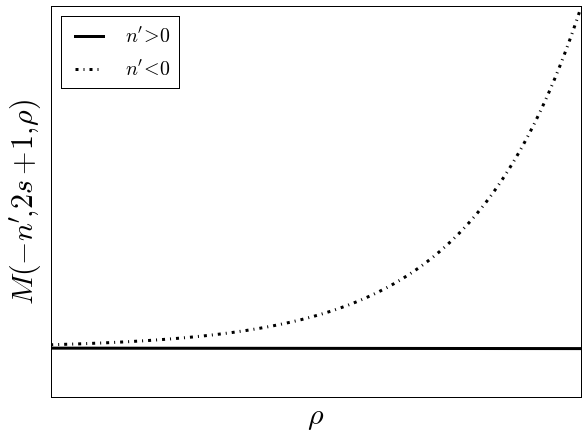
\includegraphics[scale=0.4]{hypgeo.png}
\caption*{Comportamiento asint\'otico de la funci\'on hipergeometrica.}
\label{fig:hypgeo}
\end{figure}  

Para $n' = 0$ la funci\'on hipergeometrica converge pero las funciones (\ref{eq:sol2}) y (\ref{eq:sol1})
divergen. Por lo tanto si $n'=0$ la constante $a_0 = 0$ para (\ref{eq:sol1}) y $\kappa - \xi kc / \lambda$
para (\ref{eq:sol2}), lo cual implica que para $n'=0$ $\kappa > 0$. 

\subsection{Niveles de Energ\'ia}

%------------------------------------------------APENDICE----------------------

\section{Ap\'endice: Demostraci\'ones y desarrollos matematicos}\label{sec:apendice}

\subsection{Propiedades de las matrices $\widetilde{\alpha}$, $\widetilde{\beta}$,  
$\widetilde{\sigma}$ y $\widetilde{\gamma}_5$}\label{sec:gamma5}

Las matrices $\alpha$, $\beta$ y $\sigma$ cumplen con las siguientes relaciones:

\[
\widetilde{\sigma_i}^2 = \widetilde{\mathbf{I}}
\]

\[
[\widetilde{\sigma_i}, \widetilde{\sigma_j}] = 2i\epsilon_{ijk}\widetilde{\sigma_k}
\]

\[
\{\widetilde{\sigma_i},\widetilde{\sigma_j}\} = 2\widetilde{\mathbf{I}}\delta_{ij}
\]

\[
[\widetilde{\sigma_i}, \widetilde{\alpha_i}] = 0
\]

\[
\{ \widetilde{\sigma_i}, \widetilde{\alpha_j} \} = 0;  \ i \neq j
\]

\[
\widetilde{\alpha} \times \widetilde{\alpha} = 2i\widetilde{\sigma}
\]

\[
\widetilde{\gamma}_i = \widetilde{\beta}\widetilde{\alpha}_i = 
\begin{pmatrix}
0 & \widetilde{\sigma}_i \\
-\widetilde{\sigma}_i & 0 \\
\end{pmatrix}
\]

Donde $i = x, y, z$. Adicionalmente se pueden definir las matrices $\widetilde{\gamma_4}$ y $\widetilde{\gamma_5}$


\[
\widetilde{\gamma}_4 = \widetilde{\beta}\widetilde{I} = 
\begin{pmatrix}
\widetilde{I} & 0 \\
0 & -\widetilde{I}  \\
\end{pmatrix}
\]

\begin{equation}\label{eq:gamma5}
\widetilde{\gamma}_5 = i\widetilde{\gamma}_1 \widetilde{\gamma}_2 \widetilde{\gamma}_3 \widetilde{\gamma}_4 = 
\begin{pmatrix}
0 & -\widetilde{I} \\
-\widetilde{I} & 0 \\
\end{pmatrix}
\end{equation}


\[
\widetilde{\gamma_5} = 
\begin{pmatrix} 
0 & - \widetilde{I} \\
-\widetilde{I} & 0 \\
\end{pmatrix}
\]

Donde $\widetilde{I}$ es la matriz identidad de dos dimensiones. Operando  $\widetilde{I}$ 
en $\widetilde{\alpha}$ y $\widetilde{\sigma}$ obtenemos:

\[
\widetilde{\gamma_5}\widetilde{\alpha_i} = 
\begin{pmatrix} 
0 & - \widetilde{I} \\
-\widetilde{I} & 0 \\
\end{pmatrix} 
\begin{pmatrix} 
0 & \sigma_i \\
\sigma_i & 0 \\
\end{pmatrix} 
= 
\begin{pmatrix}
-\sigma_i & 0 \\
0 & -\sigma_i
\end{pmatrix}
= -\widetilde{\sigma_i}
\]

y an\'alogamente:

\[
\widetilde{\gamma_5}\widetilde{\sigma_i} = 
\begin{pmatrix} 
0 & - \widetilde{I} \\
-\widetilde{I} & 0 \\
\end{pmatrix} 
\begin{pmatrix} 
\sigma_i & 0 \\
0 & \sigma_i  \\
\end{pmatrix} 
= 
\begin{pmatrix}
0 & -\sigma_i \\
-\sigma_i & 0 \\
\end{pmatrix}
= -\widetilde{\alpha_i}
\]

Adicionalmente las matrices $\widetilde{\gamma}$ cumplen con las siguientes
propiedades de conmutaci\'on y anticonmutaci\'on:

\[
\{ \widetilde{\gamma}_i, \widetilde{\gamma}_j \} = 0 \ i \neq j
\]

Y $\widetilde{\gamma}_5$ conmuta con $\widetilde{\alpha}_i$ y $\widetilde{\sigma}_i$: 

\[
[\widetilde{\gamma}_5, \widetilde{\alpha}_i] = [\widetilde{\gamma}_5,\widetilde{\sigma}_i] = 0
\]

\subsection{Definici\'on del operador $\hat{K}$}\label{sec:k}

\begin{equation}
\widetilde{\hat{K}} = \widetilde{\hat{L}}\cdot \widetilde{\sigma} + \hbar
\end{equation}

Con autovalor $-\hbar \kappa$ y donde $\kappa$ puede tomar los siguientes
valores:

\[ \kappa = 
\begin{cases}
-l - 1 \rightarrow j = l + 1/2  \\
l \rightarrow j = l - 1/2 \\ 
\end{cases}
\]  


\subsection{Desarrollos matematicos detallados de la \S \ref{sec:solucion}}\label{sec:pasoapaso}

\subsubsection{Cmabio de variable a $\phi_1$ y $\phi_2$}

Reemplazando (\ref{eq:cdv}) en (\ref{eq:Hrad1})  se obtiene:

\[
\lambda (k_C + W_C)^{1/2}(\phi_1 + \phi_2)e^{-\lambda r} + (k_C + W_C)^(1/2)e^{-\lambda r}\left( \dfrac{\partial \phi_1}{\partial r} 
+ \dfrac{\partial \phi_2}{\partial r} \right)
\]
\[
 = - \dfrac{\kappa}{r}  (k_C + W_C)^{1/2}(\phi_1 + \phi_2)e^{-\lambda r} 
+ (k_C + W_C)^{1/2}e^{-\lambda r} (\phi_1 + \phi_2)
\]

\[
+ \left ( W_C + \dfrac{\xi}{r} + K_C \right )(k_C - W_C)^{1/2}e^{-\lambda r}(\phi_1 + \phi_2)
\]


Dividiendo sobre $(k_C + W_C)^{1/2}e^{-\lambda r}$ y despejando $\left( \dfrac{\partial \phi_1}{\partial r} 
+ \dfrac{\partial \phi_2}{\partial r} \right)$ se encuentra lo siguiente:

\[
\dfrac{\partial \phi_1}{\partial r} + \dfrac{\partial \phi_2}{\partial r} = \lambda (\phi_1 + \phi_2) - \dfrac{\kappa}{r}(\phi_1 + \phi_2)
+\left( W_C + \dfrac{\xi}{r} + k_C  \right)(\phi_1 + \phi_2) 
\]

\begin{equation}
\dfrac{\partial \phi_1}{\partial r} + \dfrac{\partial \phi_2}{\partial r} = \left ( \lambda - \dfrac{\kappa}{r} \right ) (\phi_1 + \phi_2)
+\left( W_C + \dfrac{\xi}{r} + k_C  \right)(\phi_1 + \phi_2) 
\end{equation}

Que es la misma expresion que obtuvimos para (\ref{eq:phi1-1}). El procedimiento para llegar a (\ref{eq:phi1-1}) es el mismo que se realizo.

 
\subsubsection{Cambio de variable $\rho=2\lambda r$} 

Sumando  (\ref{eq:phi1-1}) y  (\ref{eq:phi2-1}) obtenemos:

\[
2 \lambda \dfrac{\partial \phi_1}{\partial r} = 2 \lambda^2  \phi_1 
- \dfrac{2 \kappa \lambda }{r}\phi_2 + \left( W_C + \dfrac{\xi}{r} + k_C  \right ) 
(k_C - w_C)(\phi_1 - \phi_2) 
\]

\[
- \left( W_C + \dfrac{\xi}{r} - k_C  \right )(k_C + w_C)(\phi_1 + \phi_2) 
\]

Haciendo el algebra de los dos ultimos terminos se encuentra:

\[
2 \lambda \dfrac{\partial \phi_1}{\partial r} -  2 \lambda^2  \phi_1 + 2\dfrac{\kappa \lambda}{r}\phi_2
= W_C(k_C - W_C)(\phi_1 - \phi_2) - W_C(k_C + W_C)(\phi_1 + \phi_2)
\]

\[
\dfrac{\xi}{r}(k_C - W_C)(\phi_1 - \phi_2) - \dfrac{\xi}{r}(k_C + W_C)(\phi_1 + \phi_2)
+ K_C (k_C - W_C)(\phi_1 - \phi_2) + k_C (k_C + W_C)(\phi_1 + \phi_2)
\]

Abriendo los terminos en parentesis se obtiene:

\[
2 \lambda \dfrac{\partial \phi_1}{\partial r} -  2 \lambda^2  \phi_1 + 2\dfrac{\kappa \lambda}{r}\phi_2
= 2W_Ck_C\phi_2 - 2W_C^2 \phi_1 - 2 \dfrac{\xi}{r}k_C \phi_2 - 2 \dfrac{\xi}{r}w_C \phi_1 
+ 2 k_C^2 \phi_1  + k_C w_C \phi_2
\]

Simplificando terminos obtenemos:

\[
 2 \lambda \dfrac{\partial \phi_1}{\partial r} -  2 \lambda^2  \phi_1 + 2\dfrac{\kappa \lambda}{r}\phi_2
= 2\lambda^2 \phi_1 - 2 \dfrac{\xi}{r}k_C \phi_2 - 2\dfrac{\xi}{r}W_C \phi_1
\]

dividiendo por $2$ toda la ecuacion obtenemos y organizando terminos obtenemos:

\begin{equation}
\lambda \dfrac{\partial \phi_1}{\partial r} - 2 \lambda^2 \phi_1 + \dfrac{\kappa \lambda}{r} \phi_2  + \dfrac{\xi W_C}{r} \phi_1 
+ \dfrac{\xi k_C}{r}\phi_2 = 0
\end{equation}

De manera an\'aloga restando (\ref{eq:phi1-1}) y  (\ref{eq:phi2-1}) se obtiene:

\begin{equation}
\lambda \dfrac{\partial \phi_2}{\partial r}  + \dfrac{\kappa \lambda}{r} \phi_1  - \dfrac{\xi W_C}{r} \phi_2 - \dfrac{\xi k_C}{r} \phi_1 = 0
\end{equation}

finalemnte si $\rho = 2\lambda r$ y $d\rho = 2 \lambda dr$ se obtiene:

\[
2\lambda^2 \dfrac{\partial \phi_1}{\partial \rho} - 2\lambda^2 \phi_1 + 2 \dfrac{\kappa \lambda^2 }{\rho} \phi_2 
+ 2 \dfrac{\xi W_C \lambda}{\rho}\phi_1 + 2\dfrac{\xi k_C \lambda }{\rho}\phi_2 = 0
\]

Y dividiendo sobre $2\lambda^2$:

\[
\dfrac{\partial \phi_1}{\partial \rho} = \phi_1 - \dfrac{\kappa}{\rho}\phi_2 - \dfrac{\xi W_C}{\lambda \rho }\phi_1 - \dfrac{\xi K_C}{\lambda \rho}
\phi_2 
\]

Que se puede ordenar como:

\begin{equation}
\dfrac{\partial \phi_1}{\partial \rho} = \left( 1 - \dfrac{\xi W_C}{\lambda \rho} \right) \phi_1 
- \left( \dfrac{\kappa}{\rho} - \dfrac{\xi k_C}{\lambda \rho} \right) \phi_2
\end{equation}

Que es la misma expresion en (\ref{eq:sol1}). El procedimiento es el mismo para llegar a (\ref{eq:sol2}).
% ---------------- coeficientes a_m y b_m

\subsection{Derivaci\'on de los coeficientes $a_m$ y $b_m$}

\begin{equation}\label{eq:am}
a_m(m+s) = a_{m-1} - \dfrac{Wc\xi}{\lambda}a_m - \left(\kappa + \dfrac{\xi kc}{\lambda}\right) b_m
\end{equation}

\begin{equation}\label{eq:bm}
b_m(m+s) = \left( -\kappa + \dfrac{\xi kc}{\lambda}  \right)a_m + \dfrac{Wc \xi}{\lambda}b_m
\end{equation}

Para poder estudiar bien estas relaciones veamos el caso $m=0$ que implica que $a_{m-1}$. Este 
sistema de ecuaciones tendr\'a soluciones si el determinante de los coeficientes es diferente de
cero. 

\[
\begin{vmatrix}
s + Wc \xi/\lambda & \kappa + \xi kc/\lambda \\
\kappa - \xi kc/\lambda & s-Wc \xi/\lambda \\
\end{vmatrix}
= 0
\]

Lo que implica que:

\[
s^2 - \dfrac{Wc^2 \xi^2}{\lambda^2} = \kappa^2 - \dfrac{\xi^2 kc^2}{\lambda^2}
\]

Y recordando que $\lambda^2 = kc^2 + Wc^2$ se obtiene:

\[
s = \pm \sqrt{\kappa^2 - \xi^2}
\]

Siempre se escoge el signo positivo en la soluci\'on de $s$ debido a que se debe garantizar siempre
que las ecuaciones (\ref{eq:phi1})  y (\ref{eq:phi2}) sean cuadrado integrables. Es de interes entonces
encontrar las relaciones de recurrencia para $a_m$ y $b_m$, por lo tanto se despeja $b_m/a_m$ de (\ref{eq:bm})

\begin{equation}\label{eq:ambm}
\dfrac{b_m}{a_m} = \dfrac{\kappa - \xi kc/\lambda}{Wc\xi /\lambda - m - s} = \dfrac{\kappa - \xi kc/\lambda}{n'-m}
\end{equation} 

En donde se definio $n' = Wc \xi /\lambda - s$. Reemplazando (\ref{eq:ambm}) en (\ref{eq:am}) se obtiene:

\begin{equation}\label{eq:am-1}
a_m = - \dfrac{n-m}{m(2s+m)}a_{m-1}
\end{equation} 

Que para el caso de $m=0$ se obtiene:

\begin{equation}
b_0 = \dfrac{\kappa - \xi kc/\lambda}{n'}a_0
\end{equation}

De (\ref{eq:am-1}) se puede ver que la relacion de recurrencia para $a_m$ es:

\begin{equation}
a_m = (-1)^m \dfrac{(n'-1)(n'-2)\cdot\cdot\cdot(n'-m)}{m!(2s+1)(2s+2)\cdot\cdot\cdot(2s+m)}a_0
\end{equation} 

Y con un procedimiento an\'alogo se deduce que $b_m$ es:
 
\begin{equation}
b_m = (-1)^m \dfrac{n'(n'-1)\cdot\cdot\cdot (n'-m +1)}{m!(2s+1)(2s+2)\cdot\cdot\cdot(2s+m)}b_0
\end{equation}

%	BIBLIOGRAPHY
%----------------------------------------------------------------------------------------

\bibliographystyle{plain}

\bibliography{bibliografia}

%----------------------------------------------------------------------------------------

\end{document}
